\newpage



%============================================================
\section{Slope and Flux Limiters}\label{chap:limiters}
%============================================================



%===========================================
\subsection{Why Limiters?}
%===========================================

Limiters are employed because issues arise around numerical schemes due to their discrete nature.
For example, a non-limited piecewise linear advection scheme will produce oscillations around jump discontinuities.
See \textbf{Godunov's Theorem}:



\begin{displayquote}
	Linear numerical schemes for solving partial differential equations (PDE's), having the property of not generating new extrema (monotone scheme), can be at most first-order accurate.
\end{displayquote}


So if we want to employ linear higher order schemes, we will generate new extrema, which induce non-physical extrema around steep gradients, in particular around discontinuities.
An example of the arising oscillations for linear advection is shown in fig. \ref{fig:advection-pwlin-four-shapes-fixed-positive-vel}.
Obviously, ideally we want both: High order accuracy and no unphysical oscillations.
So how do we avoid this problem?
This is where limiters enter the game.









%===========================================
\subsection{How do they work?}
%===========================================


First of all, let's try and express our criterion for the scheme not to introduce spurious oscillations mathematically.
We are looking for so called monotone schemes, which don't introduce new extrema into our data.
It can be shown\footnote{
	at least for the case of linear advection, it can be done rigorously. 
	For other conservation laws, an empirical approach is usually necessary, as proof becomes exponentially more difficult, or even impossible.
}
that monotone schemes are \textbf{Total Variation Diminishing (TVD)}.
A method is TVD if:

\begin{align}
	TV(\U^n) &\equiv \sum_j | \U_{j+1} - \U_j | && \text{ Definition: Total Variation of a state}\\
	TV(\U^{n+1}) &\leq TV(\U^n) \quad \Leftrightarrow && \text{ method is TVD }
\end{align}


How do we magic up TVD methods?
A very popular approach, perhaps the most well known one, relies on the fact that some schemes are in fact TVD, but only for certain cases, which depend on the dataset.
Commonly the dependence on the dataset is expressed through the ratio of the upwind difference to the local difference $r$:

\begin{align*}
	r^n_{i-\half} &= \begin{cases}
		\frac{\U_{i-1}^n - \U_{i-2}^n}{\U_{i}^n - \U_{i-1}^n} 	\quad \text{ for } \V  \geq 0 \\
		\frac{\U_{i+1}^n - \U_{i}^n}{\U_{i}^n - \U_{i-1}^n} 	\quad \text{ for } \V  \leq 0 \\
	\end{cases}
\end{align*}.

$r$ is  a measure of the ``curvature'', or ``monotonicity'' in that place, and called the ``flow parameter''.

Different schemes cover various ranges of values for $r$ for which they are TVD.
So the idea is as follows:
\emph{Let's use different schemes to solve our problem depending on what states we have currently present in our dataset, such that our method is always TVD.}
Which scheme we employ depends on the value of $r$, and the expressions for fluxes become non-linear because from this point on, we choose the coefficients for the fluxes\footnote{	
	the schemes will always be of the form $\U^{n+1}_i = \sum_{k = -k_L}^{k_R} \beta_{i+k} \U_{i+k}$, but from now on, $\beta = \beta(r)$
} depending on $r$.
Also remember that first-order schemes are monotone, but very diffusive and have low accuracy.
With that in mind, if nothing else works, we can still switch back to a first-order scheme only at the point where we need it.


















%=====================================================
\subsection{Constructing Limiters}
%=====================================================


In general, the limiters need to be constructed for every method differently, depending on which methods you want to switch between, how you're treating the fluxes, etc.
In any case, you start off by introducing coefficients $\phi(r)$ which depend on $r$, and then apply the TVD constraint, giving you a region in the $r-\phi(r)$ plot:
The TVD constraint gives you inequalities, thus some upper and lower limits for $\phi$ at given $r$.
Within this TVD region, a multitude of possible expressions for $\phi$ are possible.
See for example fig. \ref{fig:limiters-r-phi}, where some popular limiters are plotted within the grey TVD region.



Depending on the way you're trying to get high-order accuracy, you can have various approaches to introduce a limiter function $\phi(r)$ in your scheme:

\begin{itemize}
	\item 	If the high-order approach is to treat the states as not constant, but some higher order interpolation, e.g. piecewise linear advection, or any MUSCL scheme, then we use \emph{slope limiters} to modify the expression for the slope of the piecewise linear states such that the resulting method is TVD.
	\item 	If we leave the states constant, but use a more clever way to get fluxes, e.g. WAF schemes, then we need \emph{flux limiters} directly, as no slopes are available.
\end{itemize}

















%==========================================================
\subsection{Slope Limiters}\label{chap:slope_limiters}
%==========================================================




Let's start with slope limiters.
The idea is to compute the slope in way that is useful for us based on the current situation of the gas state that we're solving for.

The choice of the slope can be expressed via a function $\phi(r)$.
For linear advection, we are solving the equation:

\begin{align}
	\U_i ^{n+1} &= 
		\U_i^{n} +  \frac{\Delta t}{\Delta x} \left( \F_{i-\half}^{n+\half} - \F_{i+\half}^{n+\half} \right) \label{eq:advection}
\end{align}


Recall that we're working for a scalar conservation law here, and just treat every component of the state $\U$ independently.


If we assume that the states $\U_i$ are piecewise linear, i.e.
\begin{align}
	\U(x) = \U_i(x_i) + \mathbf{s}\cdot (x - x_i) \quad \text{ for } x_{i-\half} \leq x \leq x_{i+\half} \label{eq:advection-slope}
\end{align}


then the expression for the fluxes is given by


\begin{align*}
	\F_{i-\half}^{n+\half} &= 
		\begin{cases}
			v_{i-\half} \cdot \U_{i-1}^n +  \frac{1}{2} v_{i-\half} \cdot\mathbf{s}_{i-1}^n (\Delta x -  v_{i-\half} \Delta t)
			 	& \quad \text{for } v \geq 0 \\
			v_{i-\half} \cdot \U_{i}^n -\frac{1}{2} v_{i-\half} \cdot \mathbf{s}_{i}^n (\Delta x + v_{i-\half} \Delta t)
				& \quad \text{for } v \leq 0 \\
		\end{cases} \\
	\F_{i+\half}^{n+\half} &= 
		\begin{cases}
			v_{i+\half} \cdot \U_{i}^n +  \frac{1}{2} v_{i+\half} \cdot\mathbf{s}_{i}^n (\Delta x -  v_{i+\half} \Delta t)
			 	& \quad \text{for } v \geq 0 \\
			v_{i+\half} \cdot \U_{i+1}^n -\frac{1}{2} v_{i+\half} \cdot \mathbf{s}_{i+1}^n (\Delta x + v_{i+\half} \Delta t)
				& \quad \text{for } v \leq 0 \\
		\end{cases} \\		
\end{align*}




Let us introduce the unitless function $\phi(r)$ as

\begin{align}
	\phi(r_{i+\half}) &= \phi_{i+\half} = 
		\begin{cases}
			\frac{\Delta x}{\U_{i+1} - \U_{i}} \cdot \mathbf{s}_{i} 	& 	\text{ for } v \geq 0 \\
			\frac{\Delta x}{\U_{i+1} - \U_{i}} \cdot \mathbf{s}_{i+1}	&	\text{ for } v \leq 0 \\
		\end{cases}
		\\
	\phi(r_{i-\half}) &= \phi_{i-\half} = 
		\begin{cases}
			\frac{\Delta x}{\U_i - \U_{i-1}} \cdot \mathbf{s}_{i-1} 	& 	\text{ for } v \geq 0 \\
			\frac{\Delta x}{\U_i - \U_{i-1}} \cdot \mathbf{s}_{i}	&	\text{ for } v \leq 0 \\
		\end{cases}
\end{align}


Such that

\begin{align*}
	\F_{i-\half}^{n+\half} &= 
		\begin{cases}
			v_{i-\half} \cdot \U_{i-1}^n + \frac{1}{2} |v_{i-\half}|  \left(1 -  \frac{|v_{i-\half}| \Delta t}{\Delta x} \right) \phi_{i-\half} ( \U_i - \U_{i-1} )
			 	& \quad \text{for } v \geq 0 \\
			v_{i-\half} \cdot \U_{i}^n + \frac{1}{2} |v_{i-\half}|  \left(1 -  \frac{|v_{i-\half}| \Delta t}{\Delta x} \right) \phi_{i-\half} ( \U_i - \U_{i-1} )
				& \quad \text{for } v \leq 0 \\
		\end{cases} \\		
	\F_{i+\half}^{n+\half} &= 
		\begin{cases}
			v_{i+\half} \cdot \U_{i}^n + \frac{1}{2} |v_{i+\half}|  \left(1 -  \frac{|v_{i+\half}| \Delta t}{\Delta x} \right) \phi_{i+\half} ( \U_{i+1} - \U_{i} )
			 	& \quad \text{for } v \geq 0 \\
			v_{i+\half} \cdot \U_{i+1}^n + \frac{1}{2} |v_{i+\half}|  \left(1 -  \frac{|v_{i+\half}| \Delta t}{\Delta x} \right) \phi_{i+\half} ( \U_{i+1} - \U_{i} )
			 	& \quad \text{for } v \geq 0 \\
		\end{cases} \\		
\end{align*}












Depending on our choice of $\phi$, we can get different slopes, which are not limited, but well known schemes:
Here for positive velocity only, and for $r = r_{i-\half}$:

\begin{align}
	\phi(r) & = 0 \rightarrow \mathbf{s}_i = 0 
		&\text{ No slopes; Piecewise constant method.}\\
	\phi(r) & = 1 \rightarrow \mathbf{s}_i = \frac{\U_{i} - \U_{i-1}}{\Delta x} 
		&\text{ Downwind slope (Lax-Wendroff)} \\
	\phi(r) & = r \rightarrow \mathbf{s}_i = \frac{\U_{i-1} - \U_{i-2}}{\Delta x} 
		&\text{Upwind slope (Beam-Warming)} \\
	\phi(r) & = \frac{1}{2} (1 + r) \rightarrow \mathbf{s}_i = \frac{\U_{i} - \U_{i-2}}{2 \Delta x} 
		&\text{ Centered slope (Fromm)} \\
\end{align}



Note that taking the downwind slope is very different from doing downwind differencing!
We only use the downwind value to estimate the state inside the cell, not to compute derivatives.




\begin{figure}
	\centering
	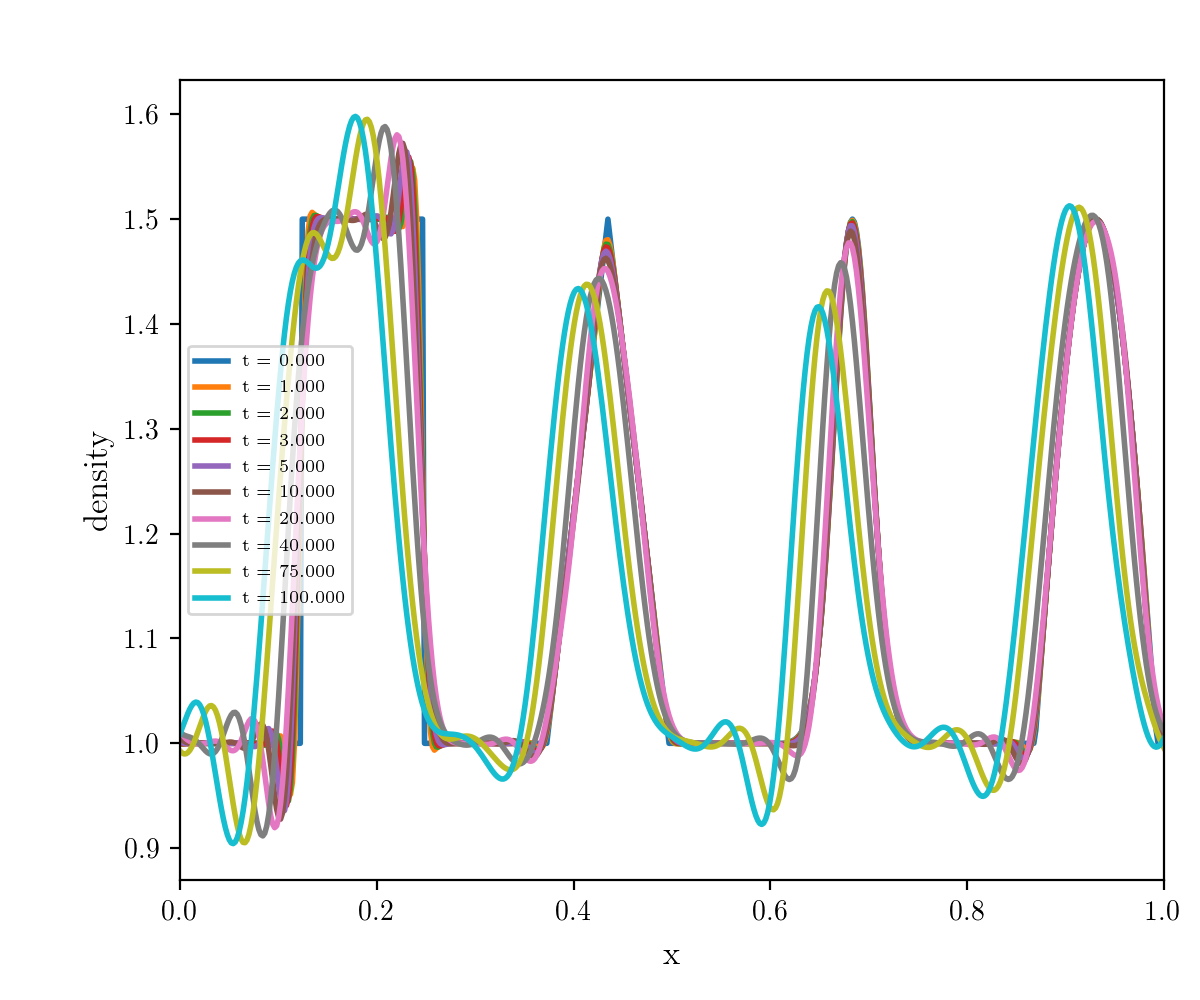
\includegraphics[width=.9\textwidth]{./figures/advection-pwlin-four-shapes.png}%
	\caption{
		\label{fig:advection-pwlin-four-shapes-fixed-positive-vel}
		Piecewise linear advection with positive fixed global velocity $v_x = 1$ at different times. 
		$C_{CFL} = 0.9$,  $nx = 100$.
		The oscillations are a natural consequence according to Godunov's theorem.
	}
\end{figure}








To remove the oscillations that we see in fig. \ref{fig:advection-pwlin-four-shapes-fixed-positive-vel}, we want to go back to a first order expression (piecewise constant expression) when we find an oscillation, i.e. when the numerator and denominator have different signs.
We get the piecewise constant expression for $\phi(r) = 0$.

$\Rightarrow$ For slope limiters, we must have $r < 0 \Rightarrow \phi = 0$


Other restrictions follow from the constraint that the method should be TVD and continuous (see \cite{swebyHighResolutionSchemes1984}):

\begin{align}
	r \le& \phi(r) \le 2r 	&&	 0  \le r \le 1 \label{eq:TVD-consequence-first}\\
	1 \le& \phi(r) \le r 	&&	 1 \le r \le 2 \\
	1 \le& \phi(r) \le 2 	&&	 r > 2 \\
	& \phi(1) = 1 &&  \label{eq:TVD-consequence-last}
\end{align}



Effectively, this defines regions in the $r-\phi(r)$ diagram through which the limiters are allowed to pass such that they are still TVD (fig \ref{fig:limiters-r-phi}).
The implemented limiters are given in section \ref{chap:implemented_limiters}.




















%===========================================================
\subsection{Flux Limiters}
%===========================================================






In general, flux limiters need to be constructed for each method individually.
There are some general approaches to help you get started, see e.g. \cite{Toro}.

Lucky for us, for linear advection, we can find relations between the slope limiters $\phi(r)$ described in section \ref{chap:slope_limiters}, while the full expressions for $\phi(r)$ are given in section \ref{chap:implemented_limiters}.





%=============================================================
\subsubsection{The limited WAF flux}
%=============================================================



For WAF advection, we have the expression for a limited flux

\begin{equation}
	\F_{i+\half}^{n+\half} =  
		\frac{1}{2} (1 + sign(v) \psi_{i+\half})\ v \U_i^n + \frac{1}{2} (1 - sign(v) \psi_{i+\half})\ v \U_{i+1}^n
\end{equation}


The choice
\begin{align*}
	\psi = |c|
\end{align*}
recovers the non-limited expression, where

\begin{align*}
	c = \frac{\Delta t v}{\Delta x}
\end{align*}


It can be shown that

\begin{equation}
	\psi_{i+\half} = 1 - ( 1 - |c|) \phi_{i+\half}(r)
\end{equation}


Some possible choices for the limiter function $\phi(r)$ are given in section \ref{chap:implemented_limiters}.













%=============================================================================
\subsection{ Implemented Limiters} \label{chap:implemented_limiters}
%=============================================================================




Some popular (and implemented) limiters are:
\begin{flalign}
	\text{Minmod} 								&&\quad \phi(r) &= \mathrm{minmod}(1, r)\\
	\text{Superbee} 							&&\quad \phi(r) &= \max(0, \min(1, 2r), \min(2, r)) \\
	\text{MC (monotonized cenral-difference)} 	&&\quad \phi(r) &= \max(0, \min ((1+r)/2, 2, 2r))\\
	\text{van Leer}								&&\quad \phi(r) &= \frac{r + |r|}{1 + |r|}
\end{flalign}

where

\begin{align}
	\mathrm{minmod}(a, b) = 
		\begin{cases}
			a	& \quad \text{ if } |a| < |b| \text{ and } ab > 0\\
			b	& \quad \text{ if } |a| > |b| \text{ and } ab > 0\\
			0	& \quad \text{ if } ab \leq 0\\
		\end{cases}		
\end{align}



The functions $\phi(r)$ are shown in fig. \ref{fig:limiters-r-phi}.



\begin{figure}[H]
	\centering
	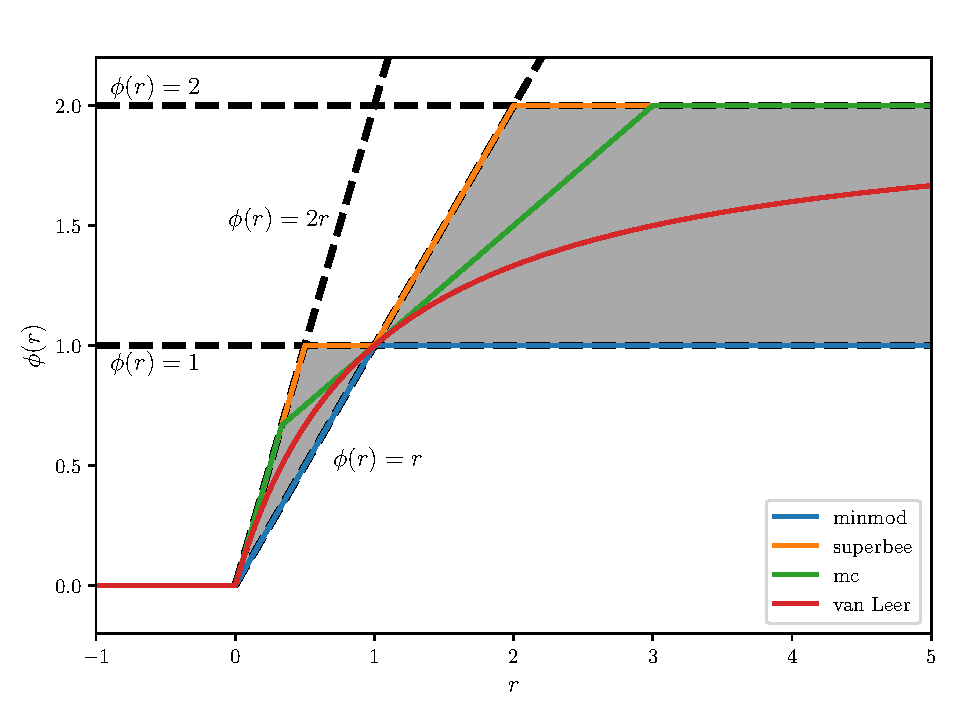
\includegraphics[width=.9\textwidth]{./figures/limiters.pdf}%
	\caption{
		\label{fig:limiters-r-phi}
		The behaviour for different slope limiters. 
		The grey zone is the zone allowed by the conditions \ref{eq:TVD-consequence-first}  - \ref{eq:TVD-consequence-last}, and is the region in which $\phi(r)$ yields a TVD method.
	}
\end{figure}
















%===========================================================
\subsection{Implementation Details}
%===========================================================


All the main functions for limiters are written in \texttt{/program/src/limiter.c} and \texttt{/program/src/limiter.h}.

If we are using slope limiters, it first finds the relevant states $\U_i$ that enter the equation, and then call a function to compute $\phi(r)$. 
The specific way how $\phi(r)$ is computed is then defined in the specific files in \texttt{/program/src/limiter/}, depending on what limiter you want.

